% !Mode:: "TeX:UTF-8" (encoding info for WinEdt)
\section{Elexis-Dignosecodes-Schweiz}
Einbindung von ICD-10 und Tessiner Code als Konsultationsdiagnosenschlüssel. Dieses Plugin ist Teil der Standard-Distribution. 

\subsection{ICD-10}
\begin{wrapfigure}{r}{7cm}
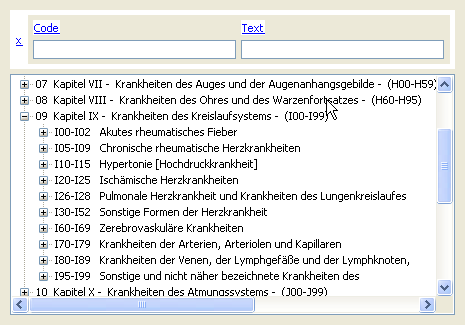
\includegraphics[width=7cm]{images/icd10}
\caption{ICD-10}
\label{fig:icd10}
\end{wrapfigure}

Das Plugin selbst enthält aber nur die Strukturen. Die Daten selbst müssen importiert werden. Weitere Erläuterungen hierzu finden Sie in \ref{config:icd10} auf S. \pageref{config:icd10}.

\medskip

ICD-10 ist ein hierarchisch aufgebauter Code. Wie Sie in \ref{fig:icd10} erkennen können, wird er in einer Baumstruktur dargestellt. Um einen Zweig zu öffnen, klicken Sie auf das kleine + Zeichen links neben dem Namen. 

In der Schweiz wird auf Tarmed- Rechnungen, die an IV, MV oder UVG-Versicherer gehen, ein ICD-10-Code als Diagnose erwartet.

\subsection{Tessiner Code (TI-Code)}
Der Tessiner Code ist ein einfacher Diagnosecode, welcher nur eine Grobspezifikation der Krankheit enthält. In der Schweiz genügt auf Tarmed-Rechnungen, die an KVG-Versicherer gehen, der TI-Code als Diagnose.

Datenimport ist nicht notwendig (Die Daten sind bereits im Plugin enthalten). Ob die deutsche, die französische oder die italienische Version des TICodes 